\documentclass{beamer}

\usepackage{default}
\usepackage{listings}
\usepackage{url}
\usepackage{tabularx}
\usepackage{multicol}


\newcommand{\rest}{REST}
\newcommand{\restful}{RESTful}
\newcommand{\restless}{RESTless}

\input{yamllang.tex}

\newcommand*{\vcenteredhbox}[1]{\begingroup
\setbox0=\hbox{#1}\parbox{\wd0}{\box0}\endgroup}

\title{Pratical \restful\ API design}
\subtitle{Exploration over technologies enabling a Model-First approach in \restful\ API development}
\author[G. Ciatto]{Giovanni Ciatto \\ \texttt{giovanni.ciatto@studio.unibo.it}}
\date{May 18, 2016}
\institute[UNIBO]{University of Bologna \\ Computer Science and Engineering}
\subject{Web Application and Services}

\usetheme{Madrid}
\usecolortheme{default}

\AtBeginSection[]
{
  \begin{frame}
    \frametitle{Table of Contents}
    \begin{multicols}{2}
    	\tableofcontents[currentsection]
    \end{multicols}
  \end{frame}
}

\AtBeginSubsection[]
{
  \begin{frame}
    \frametitle{Outline}
    \begin{multicols}{2}
   		\tableofcontents[currentsection,currentsubsection]
    \end{multicols}

  \end{frame}
}

\begin{document}

\frame{\titlepage}

\section{REST in practice}

\subsection{Overview}

\begin{frame}[allowframebreaks]
	\frametitle{Overview}

	\begin{block}{\rest\ = \textbf{RE}presentational \textbf{S}tate \textbf{T}ransfert}
	
		\begin{itemize}
		
		\item \rest\ \emph{is} basically a concept, a set of principles (best practices) referred as ``constraints'' and described through natural language
		
		\item \rest\ \emph{is not} a tight specification, and there exists more than a way to produce \restful\ web services 
			\begin{itemize} 
				\item Yeah, this is about web-services, so cool!
			\end{itemize}
			
		\item It's not a dichotomy, nor simply a matter of \restful\ and \restless\ web-services:
			\begin{itemize} 
				\item there are \emph{more \restful} ones ...
				\item ... and \emph{more \restless} ones
			\end{itemize}
			
		\item \restful\ (distributed) systems tend to be scalable, robust and easy to develop, understand and maintain
			\begin{itemize} 
				\item Yet not every system should be \restful
				\item Silver-bullets are like unicorns: they do not exist.
			\end{itemize}
		
		\end{itemize}
		
	\end{block}
	
	\begin{block}{\rest\ constraints}
		\restful\ systems *should* satisfy the following 6 constraints:
		\begin{itemize} 
			\item Client-server
			\item Stateless interaction
			\item Chaceability
			\item Uniform Interface
			\item Layered System
			\item Code on Demand (Optional)
		\end{itemize}
		 
	\end{block}

\end{frame}

\subsection{Principles}

\subsubsection{Client-server}

\begin{frame}[allowframebreaks]
	\frametitle{Client-server}
	There are two kind of entities: \emph{servers} and \emph{clients} communicating via a \emph{connector}.
	
	\begin{block}{Servers}
		Reactive entities providing one or more services to multiple clients
	\end{block}
	
	\begin{block}{Clients}
		Triggering (proactive) entities making requests that trigger reactions from servers.
	\end{block}
	
	\begin{block}{Connectors}
		Mechanism that allows communication between clients and servers (e.g. HTTP protocol, Message Oriented Middleware, RPC, etc.)
	\end{block}
	
	\framebreak

	Separation of concerns is the key concept here.
	
	\begin{block}{Separation of concerns}
		Once both clients and servers concerns have been fixed and some sort of common interface have been defined, the two kind of components evolve independently.
	\end{block}
	
	\begin{exampleblock}{Client-server constraint in web-based systems}
		Web-based systems quite often satisfy this constraint.
	\end{exampleblock}
	
\end{frame}

\subsubsection{Stateless interaction}

\begin{frame}[allowframebreaks]
	\frametitle{Stateless interaction}
	
	This is probably the most important constraint as well as the hardest one: each request from client to server must contain all of the information necessary to understand the request, and cannot take advantage of any stored context on the server. Application state is therefore kept entirely on the client.
	
	\begin{block}{Application state}
		Data that could vary by client, and per request.
	\end{block}
	
	\begin{block}{Exceptions are tolerated}
		Immutability is a utopia. For real world problems, you should just try to minimize mutability. E.g. request rate monitoring requires mutability. 
		However, make every effort to ensure that application state doesn't span multiple requests of your services.
		
	\end{block}
	
	\framebreak
	
	\begin{block}{Cookies}
		Cookies do not necessarily violate this constraint, since the are part of each HTTP interaction.
	\end{block}
	
	\begin{alertblock}{Sessions identifiers}
		Assigning any sort of temporary session identifier to the some user *and* storing session data using some data structure within server's memory is inherently a violation of the constraint.
		Since this is the common usage of cookies, they are discouraged.
	\end{alertblock}
	
	\begin{example}
		A stateless communication litmus test is to turn off session cookies, and determine if the API, web service, or web application still works as designed.
	\end{example}
	
	\framebreak
		
	\begin{block}{Authentication}
		This constraint makes authentication critical. Other approaches have been developed which are more secure and \restful. 
	\end{block}
	
	\begin{block}{Authentication over HTTP - Overview}
		\begin{itemize}
			\item HTTP\textbf{S} is base-assumption here
			\item SIDs over Cookies are stateful
			\item \emph{Basic access authentication} is conceptually what we need - too naive
			\item \emph{Digest access authentication} employs MD5...
			\item \emph{OAuth}: is strong \& complex
			\item \emph{JWT} is some good trade-off IMWO
		\end{itemize}
	\end{block}
\end{frame}

\subsubsection{Cacheability}

\begin{frame}
	\frametitle{Cacheability}
	
	\begin{block}{Cacheable responses}
		\begin{itemize}
			\item Clients can cache responses
			\item Responses must therefore, implicitly or explicitly, define themselves as cacheable, or not
			\begin{itemize}
				\item to prevent clients reusing stale or inappropriate data in response to further requests
			\end{itemize}
			\item Well-managed caching partially or completely eliminates some client-server interactions
			\begin{itemize}
				\item further improving scalability and performance
			\end{itemize}
		\end{itemize}
	
	\end{block}
\end{frame}

\subsubsection{Uniform Interface}

\begin{frame}[allowframebreaks,fragile]
	\frametitle{Uniform Interface}
	
	\begin{itemize}
		\item The uniform interface constraint defines the interface between clients and servers. 
		\item This is probably secret of \rest's simplicity and strength.
		\item \restful\ systems expose a standard, unambiguous, clear and human-readable API because of this constraint.
			\begin{itemize}
				\item Such a principle allows for model-driven approaches. 
			\end{itemize}
	\end{itemize}
	
	\begin{block}{Uniform Interface Requirements}
		\begin{itemize}
			\item Resource-based
			\item Manipulation of Resources Through Representations
			\item Self-descriptive Messages
			\item HATEOAS (dafuq ?!)
			
		\end{itemize}
	\end{block}
	
	\framebreak
	
	
	\begin{block}{Resource-Based}
		\begin{itemize}
			\item \restful\ systems handle \emph{resources}: servers host resources and clients want to CRUD them
			\begin{itemize}
				\item[$\Rightarrow$] \textbf{C}reate or \textbf{R}ead or \textbf{U}pdate or \textbf{D}elete
			\end{itemize}
			% \item Resources are not accessed (CRUDed) directly but through their representation(s)
			\item Resources have a \emph{hierarchical} nature
			\item Resources are identified and referenced by the mean of URIs
				\begin{itemize}
					\item[$\Rightarrow$] \textbf{U}niform \textbf{R}esource \textbf{I}dentifier
				\end{itemize}
			
		\end{itemize}
	\end{block}
		
	\begin{block}{HTTP Verbs}
	
		\begin{itemize}
			\item CRUD in Web-based systems means exploiting HTTP methods, which are often called ``verbs'' because of their usage within APIs:
			\begin{itemize}
				\item POST is used for resource Creation
				\item GET mean is to Read resources
				\item PUT aim is to Update resources
				\item DELETE is used to Delete resources					
			\end{itemize}
			\item HTTP Status codes and their general purpose semantics are part of the uniform interface too:
			\begin{itemize}
				\item e.g. any successful request will result in a \texttt{200:\,Ok} or \texttt{204:\,No\,Content} status code (depending on weather the response has body or not)
				\item e.g. trying to GET or DELETE any non-existent resource will result in a \texttt{404:\,Not\,Found} status code
				\item e.g. POSTing an already-existing user will result in a \texttt{409:\,Conflict} status code
			\end{itemize}
		\end{itemize}
	\end{block}
	
	\framebreak
	
	\begin{itemize}
		\item Example of resource creation: 
		\begin{itemize}
			\item we want to edit some user's username from \texttt{gciatto92} to \texttt{gciatto}
			\item suppose no authentication is needed
		\end{itemize}
	\end{itemize}
	
	\begin{alertblock}{Example of non-\restful\ approach}
		\begin{itemize}
			\item \texttt{GET http://example.com/users?\-user=gciatto92\&\-operation=changeName\&\-newName=gciatto}
			\item[]
			\item[$\times$] RPC style: the request contains the to-be-called operation
			\item[$\times$] No semantics for \texttt{GET} verb
			\item[$\times$] Which resource am I editing?
		\end{itemize}
	\end{alertblock}	
	
	\begin{exampleblock}{Example of \restful\ approach}
		\begin{itemize}
			\item \texttt{PUT http://example.com/users/gciatto92?newName=gciatto}
			\item[]
			\item[$\checkmark$] I'm editing the resource \texttt{gciatto92}, which is a user, composing the \texttt{users} resource, which represents the collection of registered users 
			\item[$\checkmark$] \texttt{PUT} verb means Update and that's what I am doing
			\item[$\checkmark$] URI queries are simply a mean for payload transport
		\end{itemize}
	\end{exampleblock}	
	
	\framebreak
	
	\begin{block}{Manipulation of Resources Through Representations}
		
		\begin{itemize}
			\item Resources are not accessed (CRUDed) directly but through their representation(s)
			\item Representations should expose resources traits to clients enabling them to do what they are allowed to, no more and no less
			\item Clients cannot make assumptions upon resources implementations, they can only exploit representations
		\end{itemize}
	\end{block}
	
	\begin{block}{Self-descriptive Messages}
			
		\begin{itemize}
			\item Each message must include enough information to describe how to process the message itself
			\begin{itemize}
				\item E.g. HTTP's \emph{Content Negotiation} is a powerfull feature: use it! \texttt{Accept} and \texttt{Content-Type} headers allow different representations for resources exposing some business logic
				\item Prefer JSON but try to support XML
			\end{itemize}
			
		\end{itemize}
	\end{block}
	
	\framebreak
	
	\begin{block}{HATEOAS - \textbf{H}ypermedia \textbf{A}s \textbf{T}he \textbf{E}ngine \textbf{O}f \textbf{A}pplication \textbf{S}tate}
			
		\begin{itemize}
			\item Difficult constraint to fully accomplish IMHO
			\item Weak definition is enough for our concerns: \emph{``Services responses should contain \emph{`relational links'} when they may be useful''}
			\item Relationships are standardized
			\item In completely-RESTful HTTP-based systems, relational links are the only mean used by clients to interact with servers
		\end{itemize}
	\end{block}
	
	\begin{example}
		\texttt{GET http://example.com/users?limit=3} \\
		supposing the first three users are \texttt{gciatto}, \texttt{mfrancia} and \texttt{mneri}, it should return something like:
		\begin{lstlisting}[basicstyle=\scriptsize]
			[
			  {
			    "username" = "gciatto",
			    "links" = [
			      { "rel" = "next", "href" = "/users/mfrancia" },
			      { "rel" = "prev", "href" = "/users/mneri" },
			      { "rel" = "first", "href" = "/users/gciatto" },
			      { "rel" = "last", "href" = "/users/mneri" },
			      { "rel" = "self", "href" = "/users/gciatto" }
			    ]
			  }
			  ...
			]
		\end{lstlisting}
	\end{example}
		
\end{frame}

\subsubsection{Layered System}

\begin{frame}
	\frametitle{Layered System}
	
	\begin{block}{Rules}
		\begin{itemize}
			\item A client cannot ordinarily tell whether it is connected directly to the end server, or to an intermediary along the way
			\item Intermediary servers may improve system scalability by enabling load-balancing and by providing shared caches
			\item Layers may also enforce security policies
		\end{itemize}
	\end{block}
	
	\begin{exampleblock}{In practice}
		\emph{DO NOT} make assumption about network topology
	\end{exampleblock}

\end{frame}

\subsubsection{Code on demand}

\begin{frame}
	\frametitle{Code on demand (optional constraint)}
	
	\begin{block}{Rules}
		\begin{itemize}
			\item Servers are able to \emph{temporarily} extend or customize the functionality of a client by transferring logic to it that it can execute
		\end{itemize}
	\end{block}
	
	\begin{exampleblock}{In practice}
		JavaScript
	\end{exampleblock}

\end{frame}


\newcommand{\swaggerlogo}{\vcenteredhbox{\includegraphics[height=0.07\textheight]{./img/tag_swagger.png}}}
\newcommand{\ramllogo}{\vcenteredhbox{\includegraphics[height=0.07\textheight]{./img/tag_raml.jpg}}}
\newcommand{\blueprintlogo}{\vcenteredhbox{\includegraphics[height=0.07\textheight]{./img/tag_apiblueprint.png}}}

\section{Model-First approach}

\subsection{Overview}

\subsubsection{Steps of REST Service Creation}

\begin{frame}[allowframebreaks]
	\frametitle{Steps of REST Service Creation}
	
	Supposing we already defined some \emph{logic architecture} of the system or we `simply' need to wrap some pre-existing SW:
	\setbeamertemplate{enumerate items}[default]
	\begin{enumerate}
		\item Define the mean(s) for user/caller authentication
		\item Identify \emph{resources} and HTTP \emph{verbs} they support
		\item Assign some \emph{route} (URI) to each resource
		\begin{itemize}
			\item Routes can contain one or more \emph{query parameters}
		\end{itemize}
		
		\framebreak
		
		\item For each method supported by each route:
		\begin{enumerate}
			\item Choose one ore more needed authentication means
			\item Define supported request/response \emph{content-types}
			\begin{itemize}
				\item \texttt{application/json}, \texttt{application/xml}, \texttt{text/html}, \ldots			
			\end{itemize}
			\item Define \emph{where} to put \emph{request's arguments}
			\begin{itemize}
				\item Headers, Body, URI, Query	
			\end{itemize}
			\item Define request's arguments \emph{structures}
			\begin{itemize}
				\item \emph{JSON Schema}, \emph{DTD}, \emph{XML Schema}, \ldots
			\end{itemize}
			\item Define \emph{status codes} allowed as \emph{responses} and, for each one:
				\begin{itemize}
					\item \emph{Body}'s structure
					\item \emph{Headers}' structure
				\end{itemize}
		\end{enumerate}
	\end{enumerate}
	
	\framebreak
	
	\begin{exampleblock}{Example: Pet Store - API Routes}
		\includegraphics[width=\textwidth]{./img/api_example_paths_alpha.png}
	\end{exampleblock}
	
	\framebreak
		
	\begin{exampleblock}{Example: Pet Store - Route Detail}
		\includegraphics[width=\textwidth]{./img/api_example_route_alpha.png}
	\end{exampleblock}
	
	\framebreak
			
	\begin{exampleblock}{Example: Pet Store - JSON Schemas (Tiping)}
		\begin{tabularx}{\textwidth}{X||X}
			\includegraphics[width=0.48\textwidth]{./img/api_example_schemas1_alpha.png} &
			\includegraphics[width=0.48\textwidth]{./img/api_example_schemas2_alpha.png}
		\end{tabularx}
	\end{exampleblock}
	
\end{frame}

\subsubsection{Model-first tools}

\begin{frame}[allowframebreaks]
	\frametitle{Model-first tools}
	
	What if we had some formal way to model APIs?
	
	\begin{exampleblock}{Swagger}
		 \swaggerlogo\ \url{http://swagger.io}
	\end{exampleblock}
	
	\begin{exampleblock}{RAML - \textbf{R}ESTful \textbf{A}PI \textbf{M}odelling \textbf{L}anguage}	
		\ramllogo\ \url{http://www.raml.org}
	\end{exampleblock}
	
	\begin{exampleblock}{Api Blueprint}
	 	\blueprintlogo\ \url{https://apiblueprint.org/}
	\end{exampleblock}
	
	\framebreak
	
	\begin{block}{Desired facilities}
		\begin{description}
			\item[Specification Language :] allows formal (machine-readable) and intellegible (human-readable) API specification
			\item[API Console :] some sort of GUI allowing for APIs navigation (usually Web-based)
			\item[Mock server :] proxy server whose code is generated using some formal specification; it validates clients' requests and forwards them to some other server responsible for business-logic implementation
			\item[Server stub :] code stubs generated using some formal specification for some particular platform (e.g. \texttt{express-js}); clients' requests validation is performed by the generated code, programmers only have to implement business-logic
			\item[] \ldots
		\end{description}
	\end{block}
\end{frame}

\subsubsection{Users Example}

\begin{frame}[allowframebreaks]
	\frametitle{Users Example}
	
	In order to compare the three technologies the `Users' minimal API has been modelled using each language.
	
	\begin{block}{Resources and methods informal description pt. 1}
		\begin{description}
			\item[\texttt{/users} :] The set of registered users
			\begin{description}
				\item[\texttt{GET} :] Retrieves public informations for a number of users
				\item[\texttt{POST} :] Creates one user
			\end{description}
			\item[\texttt{/users/\{username\}} :] The specific user whose username is specified within the path
			\begin{description}
				\item[\texttt{GET} :] Retrieves informations about the specific user \emph{[requires authentication]}
			\end{description}
		\end{description}
	\end{block}
	
	\framebreak
	
	\begin{block}{Resources and methods informal description pt. 2}
		\begin{description}
			\item[\texttt{/users/\{username\}/token} :] The authentication token for a specific user
			\begin{description}
				\item[\texttt{POST} :] Creates and returns one signed JWT if the provided username and password (within request's body) are correct
			\end{description}
		\end{description}
		\vspace{5mm}
		\begin{itemize}
			\item Authentication: signed JWT within the \texttt{Authorization} header identifies the users 
			\item It's an example! Let's suppose HTTP it's secure.
		\end{itemize}
	\end{block}
	
	
	
\end{frame}

\subsection{Swagger}

\subsubsection{Features}

\begin{frame} %[allowframebreaks]
	\frametitle{Swagger features}
	
	\begin{itemize}
		\item[$\checkmark$] JSON/YAML-based specification language
		\begin{itemize}
			\item[$\times$] a little verbose
		\end{itemize} 
		\item[$\checkmark$] Allows to easily define type schemas
		\item[$\times$] Only explicitly supports Basic authentication, Api Key and OAuth2
		\item[$\checkmark$] Largest and most active developers community
		\item[?] Industry Backing: Reverb, 3Scale, Apigee (NFI)
		\item[$\checkmark$] Largest platform support (Clojure, Go, JS, Java, Node, .Net, PHP, Python, Ruby, Scala)
		\item[$\checkmark$] Web-based editor (API console included) available at \url{http://editor.swagger.io} or as \texttt{nodejs} module
		\item[$\checkmark$] Generates extremely detailed API which allows for in-app testing
		\begin{itemize}
			\item[$\times$] not-so-easy setup: it's a standalone server
		\end{itemize} 
		\item[$\checkmark$] Lots of tools for editing (\texttt{Swagger Editor}), code generation (\texttt{Swagger Codegen}) or API presentation/navigation (\texttt{Swagger UI})
	\end{itemize}
\end{frame}

\subsubsection{Users example}

\begin{frame}[allowframebreaks,fragile]
	\frametitle{Swagger - Users example}
	\begin{exampleblock}{Headers}
		\begin{lstlisting}[language=yaml,basicstyle=\tiny,linewidth=0.48\textwidth] 
			swagger: '2.0'
			info:
			  description: Some description here
			  version: 16.05 acute angle
			  title: Swagger Sample App
			  contact: 
			    name: gciatto
			    email: giovanni.ciatto@gmail.com
			tags:
			  - name: Users
			  - name: Default  
			securityDefinitions:
			  JWT-User:
			    type: apiKey
			    in: header
			    name: Authorization
			    x-jwt-header:
			      alg: HS512
			    x-jwt-payload:
			      iss: localhost
			      aud: localhost
			      role: user
			schemes:
			  - http
		\end{lstlisting}
	\end{exampleblock}
	
	\begin{exampleblock}{JSON Schemas definitions (2 columns)}
		\begin{columns}
		\begin{column}{0.48\textwidth}
		\begin{lstlisting}[language=yaml,basicstyle=\tiny] 
			definitions:
			  Error:
			    type: object
			    required:
			      - message
			      - status
			    properties:
			      message:
			        type: string
			      status:
			        type: integer
			        format: int32
			  Token:
			    type: object
			    required:
			      - token
			    properties:
			      token:
			        type: string
			  User:
			    type: object
			    required:
			      - admin
			      - username
		\end{lstlisting}
		\end{column}
		\begin{column}{0.48\textwidth}	
		\begin{lstlisting}[language=yaml,basicstyle=\tiny] 
			    properties:
			      admin:
			        type: boolean
			        default: false
			      name:
			        type: string
			      surname:
			        type: string
			      username:
			        type: string
			  UserAuth:
			    type: object
			    required:
			      - password
			      - username
			    properties:
			      password:
			        type: string
			      username:
			        type: string
		\end{lstlisting}
		\end{column}
		\end{columns}
	\end{exampleblock}
	
	\begin{exampleblock}{Paths (columns 1-2 / 4)}
		\begin{columns}
		
		\begin{column}{0.48\textwidth}
		\begin{lstlisting}[language=yaml,basicstyle=\tiny]
			paths:
			  /users:
			    get:
			      tags:
			        - Users
			      operationId: getUsers
			      consumes: []
			      produces:
			        - application/json
			      parameters:
			        - name: limit
			          in: query
			          required: false
			          type: integer
			          format: int64
			          x-example: 10
			        - name: offset
			          in: query
			          required: false
			          type: integer
			          format: int64
			          x-example: 0
			      responses:
		\end{lstlisting}
		\end{column}
		
		\begin{column}{0.48\textwidth}
		\begin{lstlisting}[language=yaml,basicstyle=\tiny]
			        '200':
			          description: |
			            The request has succeeded
			          schema:
			            $ref: '#/definitions/User'
			    post:
			      tags:
			        - Users
			      operationId: postUsers
			      consumes: []
			      produces: []
			      parameters: []
			      responses:
			        '200':
			          description: OK
			  '/users/{username}':
			    get:
			      tags:
			        - Users
			      consumes: []
			      produces:
			        - application/json
			      parameters:
		\end{lstlisting}
		\end{column}
		
		\end{columns}
	\end{exampleblock}
	
\begin{exampleblock}{Paths (columns 3-4 / 4)}
		\begin{columns}
		
		\begin{column}{0.48\textwidth}
		\begin{lstlisting}[language=yaml,basicstyle=\tiny]
			        - name: username
			          in: path
			          required: true
			          type: string
			      responses:
			        '200':
			          description: Success
			          schema:
			            $ref: '#/definitions/User'
			        '401':
			          description: Error 401
			          schema:
			            $ref: '#/definitions/Error'
			        '404':
			          description: Error 404
			          schema:
			            $ref: '#/definitions/Error'
			      security: 
			        - JWT-User: []
			  '/users/{username}/token':
			    post:
			      tags:
			        - Users
		\end{lstlisting}
		\end{column}
		
		\begin{column}{0.48\textwidth}
		\begin{lstlisting}[language=yaml,basicstyle=\tiny]
			      consumes:
			        - application/json
			      produces:
			        - application/json
			      parameters:
			        - name: username
			          in: path
			          required: true
			          type: string
			        - in: body
			          name: body
			          required: false
			          schema:
			            $ref: '#/definitions/UserAuth'
			      responses:
			        '200':
			          description: Success
			          schema:
			            $ref: '#/definitions/Token'
			        '401':
			          description: Error 401
			          schema:
			            $ref: '#/definitions/Error'
		\end{lstlisting}
		\end{column}
		
		\end{columns}
	\end{exampleblock}

\end{frame}

\subsubsection{How to `run' the example}

\begin{frame}
	\frametitle{Swagger - How to `run' the example}
	
	\setbeamertemplate{enumerate items}[default]
	\begin{enumerate}
		\item Open some web browser and go to \url{http://editor.swagger.io}
		\item Copy \& paste the YAML code
		\begin{itemize}
			\item Pay attention to indentation!
		\end{itemize}
		\item As you will notice, the API console on the right allows you to navigate the specification
		\item The \texttt{`Generate Server'} allows you to generate the server's stub
		\item Refer to \url{http://swagger.io/open-source-integrations/} to see the complete tools gamma
	\end{enumerate}
\end{frame}

\subsection{RAML}

\subsubsection{Features}

\begin{frame} %[allowframebreaks]
	\frametitle{RAML features}
	
	\begin{itemize}
			\item[$\checkmark$] YAML-based specification language
			\begin{itemize}
				\item[$\times$] for more concise than Swagger
			\end{itemize} 
			\item[$\times$] RAML v. 0.8 uses raw JSON-Schemas (very verbose)
			\item[$\checkmark$] Supports Basic \& Digest authentication, OAuth 1 \& 2 and explicitly supports custom authentication
			\item[$\times$] Poor community support
			\item[$\checkmark$] Largest industry Backing: MuleSoft, SOA, AngularJS, Intuit, Box, PayPal \& Programmable Web
			\item[$\checkmark$] Large platform support (JavaScript, Java, Node, PHP, Python, Ruby)
			\begin{itemize}
				\item[$\times$] v. 1.0 is still poorly supported
			\end{itemize} 
			\item[$\checkmark$] Editor plugin for Atom IDE (API console included) 
			\item[$\checkmark$] Generates easy-to-read API into a single \texttt{.html} or \texttt{.md} file through some community tool
			\item[$\times$] Too much community (poorly supported) tools
		\end{itemize}
\end{frame}

\subsubsection{Users example}

\begin{frame} %[allowframebreaks]
	\frametitle{RAML - Users example}
	
	\begin{alertblock}{TODO}
		Insert example here
	\end{alertblock}
\end{frame}

\section{Authentication}

\subsection{JWT: JSON Web Tokens}

\subsubsection{Overview}

\begin{frame}[allowframebreaks]
	\frametitle{Overview}
	
	\begin{block}{JWT\emph{s} = \textbf{J}SON \textbf{W}eb \textbf{T}oken\emph{s}}
		\begin{itemize}
			\item Simple and stateless mean to provide authentication
			\begin{itemize}
				\item the server doesn't need to store session data
			\end{itemize}
			\item Use case:
			\setbeamertemplate{enumerate items}[default]
			\begin{enumerate}
				\item Some client POSTs username \& password to some predefined route, e.g. \texttt{/users/\{username\}/login}
				\item On valid requests, the server responds with one \emph{token}
				\begin{itemize}
					\item[N.B.] the token is \emph{signed} using some secret that never leaves the server, so the token \textbf{cannot be compromised or forged}
				\end{itemize}
				\item The client stores the token, e.g. within its \emph{local storage}
				\item Any subsequent request from the client should contain the token, e.g. within the \texttt{Authorization} header, the query or the body
				\item The server should verify the signature of every request containing one token: once validated, any \emph{claim} contained within the token can be entrusted
			\end{enumerate}
		\end{itemize}
		
	\end{block}
	
	\begin{block}{JWT - Sequence Diagram}
		\includegraphics[width=\textwidth]{img/jwt-diagram.png}
	\end{block}
	
\end{frame}

\subsubsection{Structure}

\begin{frame}[allowframebreaks]
	\frametitle{JWT Structure}
	
	\begin{block}{JWT - Anathomy Diagram}
		\centering
		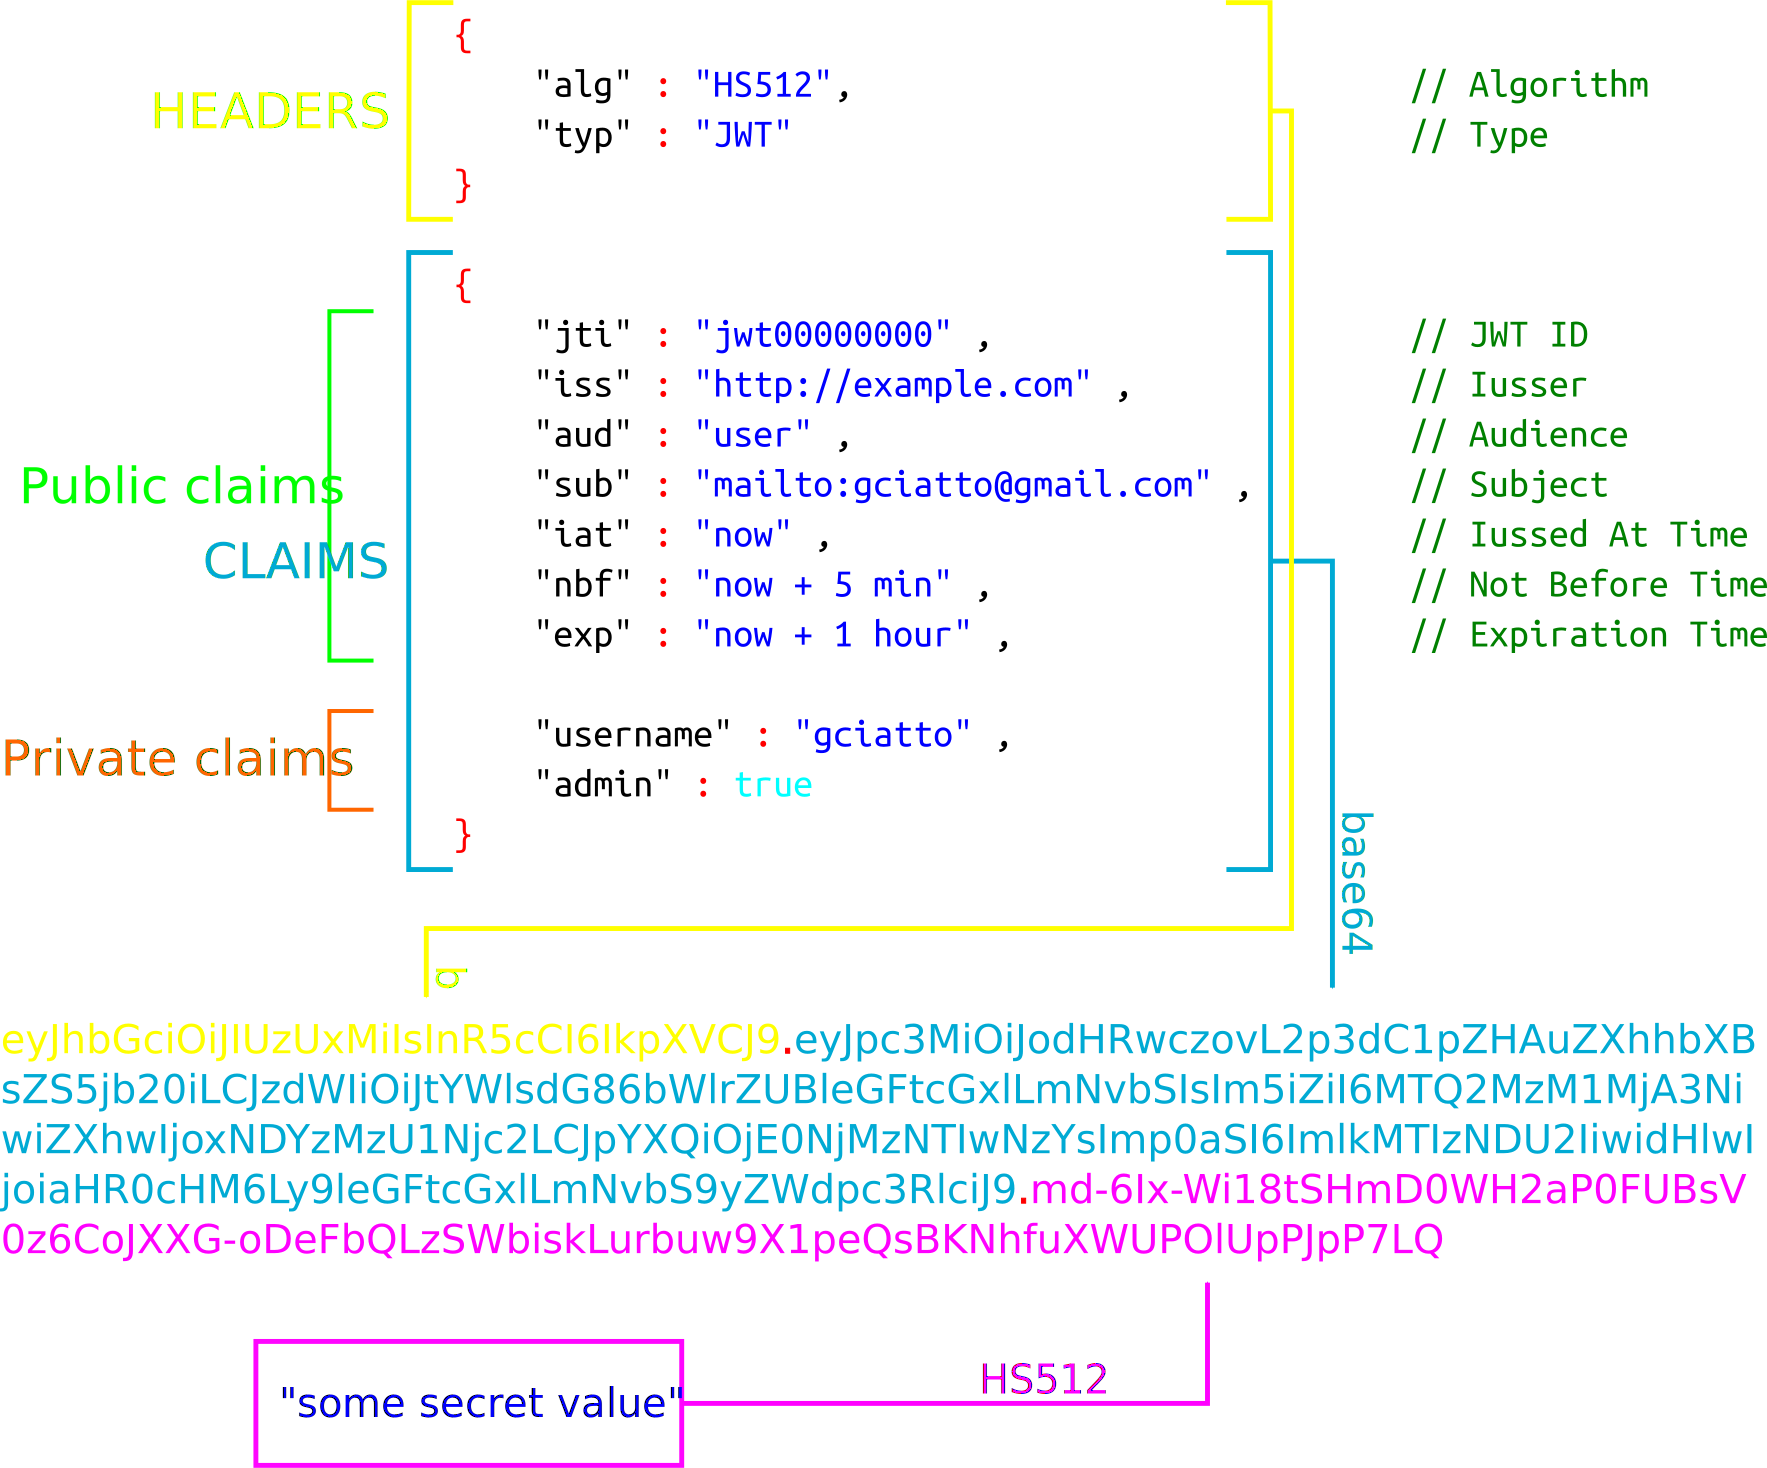
\includegraphics[height=0.7\textheight]{img/jwt.png}
	\end{block}
	
	\framebreak
	
	\begin{block}{JWT - Sections}
		\begin{itemize}
			\item Defined in \texttt{RFC 7519}
			\item String containing 3 dot-separated section
				\setbeamertemplate{enumerate items}[default]
				\begin{enumerate}
					\item The first section is a JSON object, called \emph{Headers}, \texttt{base64} encoded
					\item The second section is a JSON obect, called \emph{Claims}, \texttt{base64} encoded
					\item The third section is the \emph{Signature}, obtained using \texttt{HMAC} and some \emph{secret} string
				\end{enumerate}
		\end{itemize}
	\end{block}
	
	\begin{block}{JWT - Headers}
		\begin{description}
			\item[\texttt{typ}] (Type) : usually \texttt{"JWT"} 
			\item[\texttt{alg}] (Algorithm) : the hash algorithm used (\texttt{HS512} = \texttt{H}MAC \texttt{S}HA 512)
		\end{description}
	\end{block}
	
	\begin{block}{JWT - Public claims}
		\begin{description}
			\item[\texttt{jti}] (JWT Identifier) : identifies the entity that issued the JWT
			\item[\texttt{iss}] (Issuer) : URI of the entity issuing the token
			\item[\texttt{aud}] (Audience) : identifies the recipients that the JWT is intended for
			\item[\texttt{sub}] (Subject) : identifies the entity that is the subject of the JWT
			\item[\texttt{iat}] (Issued At) : identifies the time at which the JWT was issued
			\item[\texttt{nbf}] (Not Before) : identifies the time before which the JWT \emph{musth not} be accepted for processing
			\item[\texttt{exp}] (Expiration) : identifies the expiration time on or after which the JWT \emph{musth not} be accepted for processing
		\end{description}
	\end{block}
	
	\begin{block}{JWT - Private claims}
		\begin{itemize}
			\item They are user-defined claims
			\item REMEMBER: they are public (since the token is not encrypted) but trusted (since they are signed)
			\item E.g., within the image both username and privilege level are claimed
		\end{itemize}
	\end{block}
	
\end{frame}



\begin{frame}[allowframebreaks]
  	\frametitle<presentation>{Further Reading}    
  	
	\begin{thebibliography}{10}    
	\beamertemplatebookbibitems
	\bibitem{Fielding00}
    Fielding, Roy Thomas 
    \newblock {\em Architectural Styles and the Design of Network-based Software Architectures}.
	\newblock Doctoral dissertation, University of California, Irvine, 200.
	\newblock {\url{http://www.ics.uci.edu/~fielding/pubs/dissertation/rest_arch_style.htm}}
 	% tex.stackexchange.com/questions/68080/beamer-bibliography-icon
	\setbeamertemplate{bibliography item}[online]
    \bibitem{RestApiTutorial}
    Learn REST: A RESTful Tutorial
    \newblock {}
	\newblock {\url{http://www.restapitutorial.com/}}
	\end{thebibliography}
\end{frame}

\end{document}
